\documentclass[11pt]{article}
\usepackage[a4paper,margin=0.7in,footskip=.5cm]{geometry}
\usepackage[utf8]{inputenc}
\usepackage{amssymb} % Maths
\usepackage{amsthm} % Maths
\usepackage{amsmath} % Maths
\usepackage{graphicx} % Graphics
\usepackage{tikz-cd} % Commutative diagrams
\usepackage{amstext} % Math tables
\usepackage{array} % Math tables
\usepackage{cite} %Citations

%Theorems and Definitions
\newtheorem{definition}{Definition}
\newtheorem{theorem}{Theorem}
\newtheorem{lemma}{Lemma}
\newtheorem{proposition}{Proposition}
\newtheorem{corollary}{Corollary}
%Calculus
\newcommand{\dd}{\; \mathrm{d}}
\newcommand{\integral}[4] {\int \limits_{#1}^{#2} #3 \: \mathrm{d}#4}
\newcommand{\integ}[2]{\int\limits_{#1}^{#2}}
\newcommand{\inftyint}{\int\limits_{-\infty}^{\infty}}
\newcommand{\nsum}[2]{\sum\limits_{#1 = #2}^{\infty}}
%More Calculus
\newcommand{\pd}[2]{\frac{\partial #1}{\partial #2}}
\newcommand{\pdt}[2]{\frac{\partial^2 #1}{\partial {#2}^2}}
\newcommand{\der}[2]{\frac{\dd #1}{\dd #2}}
\newcommand{\dash}{^{\prime}}
\newcommand{\ddash}{^{\prime\prime}}
%Number sets
\newcommand{\reals}{\mathbb{R}}
\newcommand{\nats}{\mathbb{N}}
\newcommand{\integers}{\mathbb{Z}}
\newcommand{\complex}{\mathbb{C}}
\newcommand{\rationals}{\mathbb{Q}}
\newcommand{\quat}{\mathbb{H}}
\newcommand{\field}{\mathbb{F}}
%Common math commands
\newcommand{\br}[1]{\left( #1 \right)}
\newcommand{\bff}[1]{\mb{#1}}
\newcommand{\e}[1]{\mathrm{e}^{#1}}
%More common math commands
\newcommand{\scr}[1]{\mathcal{#1}}
\newcommand{\hf}{\frac{1}{2}}
\newcommand{\del}{\nabla}
\newcommand{\mo}[1]{\left| #1 \right|}
\newcommand{\cross}{\times}
\newcommand{\sqbr}[1]{\left[ #1 \right]}
\newcommand{\cbr}[1]{\left\{ #1 \right\}}
\newcommand{\angl}[1]{\langle #1 \rangle}
\newcommand{\unit}[1]{\hat{\bff{#1}}}
\newcommand{\conj}{^{*}}
\newcommand{\osum}{\oplus}
\newcommand{\bigosum}{\bigoplus}
\DeclareMathOperator*{\Res}{Res}
%Environment shortcuts
\newcommand{\eqn}[1]{\begin{align*} #1 \end{align*}}
\newcommand{\eqnstar}[1]{\begin{align} #1 \end{align}}
\newcommand{\prop}[1]{\begin{proposition} #1 \end{proposition}}
\newcommand{\thm}[1]{\begin{theorem} #1 \end{theorem}}
\newcommand{\prf}[1]{\begin{proof} #1 \end{proof}}
\newcommand{\m}[1]{\br{\begin{matrix} #1 \end{matrix}}}
\newcommand{\aray}[1]{ \left\{\begin{array}{ccc}#1\end{array}\right.}
%Misspellings
\newcommand{\detla}{\delta}
\newcommand{\simga}{\sigma}

\title{\textbf{$\scr{ANUMS}$ \LaTeX\ Workshop II}}
\author{Maxim Jeffs}
\date{\today}

\begin{document}
\maketitle

This session outlines a number of useful tools for working with \LaTeX\ -- feel free to skip to those sections that interest you. The sections primarily give brief introductions to the possibilities along with references to resources for learning more, rather than attempting to be comprehensive. As before, the source file is available on GitHub (\verb$github.com/MaximJeffs/LaTeX$). You will also need to download the bibliography file.

\section{Equation alignment with \texttt{amsmath}}

Typesetting long equations or equations broken across lines is somewhat problematic. The package \texttt{breqn} \textit{attempts} to do this automatically, but does not usually succeed, so it is typically necessary to do this manually using the \verb$amsmath$ package. If you wish to typeset a long equation or a collection of several equations, begin with the commands \verb$\begin{align}$ and \verb$\end{align}$. Adding mathematics inside the \texttt{align} environment works just as with adding entries to a matrix: use \verb$&$ to change column and \verb$\\$ to change row. For instance
\begin{verbatim}
\begin{align}
x  &= y  + z  &  j  & = k \\
   &= p  + q & \ell & = m\\
\end{align}
\end{verbatim}
will produce
\eqn{
x  &= y  + z  &  j  & = k \\
    & = p  + q  & \ell & = m\\
}
For much more on equation alignment see: 
\begin{itemize}
\item The page at \verb$www.sharelatex.com/learn/Aligning_equations_with_amsmath$, which compares multiple different methods for alignment;
\item The outline in \verb$en.wikibooks.org/wiki/LaTeX/Advanced_Mathematics$, which also includes many other important tools;
\item Or the extremely comprehensive \verb$ctan.unsw.edu.au/info/math/voss/mathmode/Mathmode.pdf$. 
\end{itemize} 

(Note that lists such as the above can be created using \verb$ \begin{itemize} \item Item one \end{itemize}$.)

\section{Figures with \texttt{graphicx}}

Inserting figures into \LaTeX\ documents is fairly easy using \texttt{graphicx}; begin by adding \verb$\usepackage{graphicx}$ to the start of the document, and the image, as a PDF file to the same folder as your \verb$.tex$ document, with file name, for instance \verb$example.pdf$. The commands
\begin{verbatim}
\begin{figure}
\centering
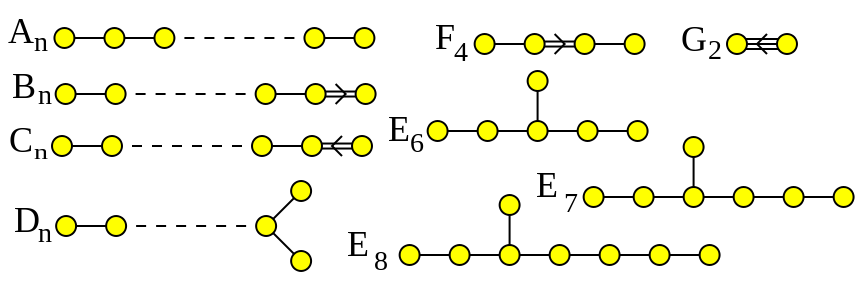
\includegraphics[width=0.6\textwidth]{example.pdf}
\caption{An example figure, courtesy of Wikipedia.}
\label{example}
\end{figure}
\end{verbatim}
will then produce Figure 1 below. Note that the \verb$width$ of the figure can be set to any multiple of the width of the text, simply by changing the number in front of \verb$\textwidth$. The \verb$\label$ command allows you to refer to the figure later in the document by typing ``See \verb$\ref{example}$'', to produce ``See Figure \ref{example}''. This can be very helpful when you have a large number of figures whose order is likely to change during the course of writing.
\paragraph{}

\begin{figure}[h]
\centering
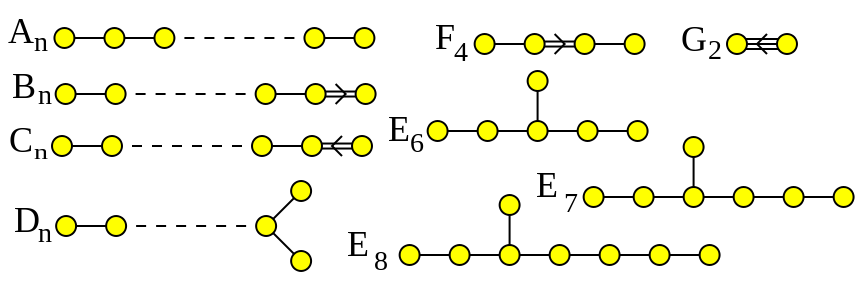
\includegraphics[width=0.6\textwidth]{example.png}
\caption{An example figure, courtesy of Wikipedia.}
\label{example}
\end{figure}

So long as you choose to compile with \texttt{PDFLaTeX}, your image file can be in any of the common image formats, such as \texttt{PNG}, \texttt{JPG} or \texttt{PDF}. However, it is recommended that you only include graphics that are in a vector format, such as \texttt{PDF}. The program InkScape is very useful for creating PDF mathematical figures and can be downloaded from \verb$inkscape.org/en/download/$. The pages at \verb$inkscape.org/en/learn/$ may also be helpful.
\paragraph{}
 One point to be wary of is that \LaTeX\ will decide for itself where to put your figure; although it is usually fairly good, it may end up putting your figure several pages after you reference it. If this is the case, try placing \verb$[h]$ after \verb$\begin{figure}$, and this will force the figure to be placed as close as possible to the location in the text.  It should be noted however that this is not always considered to be best practice; if this really concerns you, see the extremely long answer at \verb$tex.stackexchange.com/questions/39017$.

\section{Macros with \texttt{newcommand}}

Adding new commands can make typesetting mathematical documents much faster. To create a simple new command, add \verb$\newcommand{name}{what you want it to do}$ to the beginning of your document, after the \verb$\usepackage$ commands. You can then use \verb$\name$ to insert the command you have written. For example
\begin{verbatim}
\newcommand{\glnr}{ $\mathrm{GL}_{n}(\mathbb{R})$ }
\end{verbatim}
allows one to type \verb$\glnr$ in text and produce $\mathrm{GL}_{n}( \mathbb{R})$. It is also possible to create new commands with \textit{arguments}, using the code \verb$\newcommand{name}[n]{thing involving n inputs, referenced by #i}$. For instance, writing
\begin{verbatim}
\newcommand{\pd}[2]{\frac{\partial #1}{\partial #2}}
\end{verbatim}
allows one to type \verb$\pd{x}{y}$ inside an equation and produce $\pd{x}{y}$. One can also have more sophisticated examples:
\begin{verbatim}
\newcommand{\matrix}[1]{ \left( \begin{matrix} #1 \end{matrix} \right)}
\end{verbatim}
which will create a matrix inside an equation, into which you can enter entires as usual. One other useful feature is \verb$\let$, which allows you to change the default commands. For instance
\begin{verbatim}
\let\varepsilon\epsilon
\let\epsilon\varepsilon
\end{verbatim}
will change \verb$\epsilon$ to produce $\varepsilon$ instead of $\epsilon$. Finally, \verb$\DeclareMathOperator$ allows one to define `operators', such as
\begin{verbatim}
\DeclareMathOperator*{\Res}{Res}
\end{verbatim}
so that
\begin{verbatim}
\Res_{z = 1} \sum_{n=1}^{\infty} \frac{1}{n^{z}} = 1
\end{verbatim}
produces
\eqn{
\Res_{z = 1} \sum_{n=1}^{\infty} \frac{1}{n^{z}} = 1
}
Other useful types of new commands may can be found at \texttt{en.wikibooks.org/wiki/LaTeX/Macros}, such as \verb$\newenvironment$ and so forth; you can even write new commands that perform arithmetic operations on their arguments, as well as conditionals and loops!

\section{Theorems with \texttt{amsthm}}

The Definition-Theorem-Proof format of mathematical papers is easy to achieve in \LaTeX. Begin by adding \verb$\usepackage{amsthm}$ at the beginning of your document, as well as the following incantation
\begin{verbatim}
\newtheorem{theorem}{Theorem}
\newtheorem{definition}{Definition}
\end{verbatim}
Now automatically numbered Theorems and Definitions an be created by typing into a \verb$\begin{theorem} \end{theorem}$ environment, and proofs with \verb$\begin{proof} \end{proof}$. For instance,
\begin{verbatim}
\begin{definition}
A group is said to be \textbf{simple} if it has no proper non-trivial normal subgroups. 
\end{definition}
\begin{theorem}
The only finite non-trivial abelian simple groups are of prime order.
\end{theorem}
\begin{proof}
Trivial.
\end{proof}
\end{verbatim}
produces
\begin{definition}
A group is said to be \textbf{simple} if it has no proper non-trivial normal subgroups. 
\end{definition}
\begin{theorem}
The only finite non-trivial abelian simple groups are of prime order.
\end{theorem}
\begin{proof}
Trivial.
\end{proof}

Lemmas, Propositions, Corollaries, Remarks etc. may be added in the same fashion; referencing theorems may also be done with the \verb$\label$ and \verb$\ref$ commands described in Section 2. For more on the possibilities of \texttt{amsthm}, including customisation of styles and numbering, see for instance \verb$en.wikibooks.org/wiki/LaTeX/Theorems$.

\section{Diagrams with \texttt{tikz-cd}}

The package \texttt{tikz} is a general drawing package with wide capabilities; \texttt{tikz-cd} is a variant of \texttt{tikz} that is particularly useful for drawing commutative diagrams. The language works in a similar way to that for matrices except that you may produce arrows using the command \verb$\arrow{direction}{name}$. This is perhaps best illustrated through a simple example: 
\begin{verbatim}
\begin{center}
\begin{tikzcd}
A  \arrow{r}{\phi} \arrow{d}{\pi}  & B \\
A/\ker(\phi) \arrow[dashed]{ru}[swap]{\exists! \tilde{\phi}} 
\end{tikzcd}
\end{center}
\end{verbatim}
will produce

\begin{center}
\begin{tikzcd}
A  \arrow{r}{\phi} \arrow{d}{\pi}  & B \\
A/\ker(\phi) \arrow[dashed]{ru}[swap]{\exists!\tilde{\phi}} 
\end{tikzcd}
\end{center}

The best part about \texttt{tikz-cd} is the ease with which it allows you to produce all manner of strange arrows:

\begin{verbatim}
\begin{center}
\begin{tikzcd}
A\arrow[bend left]{drr}{x}
\arrow[bend right]{ddr}[swap]{y}
\arrow[dotted]{dr}[description]{(x,y)} & & \\
& B \arrow[hook]{r}{p} \arrow[two heads]{d}{q} & C \arrow{d}{f} \\
& D \arrow[bend right]{r}{g} & E
\end{tikzcd}
\end{center}
\end{verbatim}
produces

\begin{center}
\begin{tikzcd}
A\arrow[bend left]{drr}{x}
\arrow[bend right]{ddr}[swap]{y}
\arrow[dotted]{dr}[description]{(x,y)} & & \\
& B \arrow[hook]{r}{p} \arrow[two heads]{d}{q} & C \arrow{d}{f} \\
& D \arrow[bend right]{r}{g} & E
\end{tikzcd}
\end{center}

The introduction at \texttt{www.jmilne.org/not/Mtikz.pdf} is very helpful and contains a wealth of examples, as well as a nice comparison of the different packages for drawing commutative diagrams. The general \texttt{tikz} language is far more complicated: see for instance \verb$cremeronline.com/LaTeX/minimaltikz.pdf$ for an excellent short introduction. If you are not planning on creating anything terribly complicated, TikzEdt at \verb$www.tikzedt.org/$ allows you to draw a diagram and convert it into Tikz code. Unfortunately, there is currently no version for OS X, and the user must be warned that it is quite unpolished. The website \verb$www.texample.net/tikz/examples/$ is also extremely helpful if you can find a similar diagram and modify it. You are also warned in advance that tikz-cd does not always interact well with the \texttt{proof} environment. 

\section{Referencing with \texttt{bibtex}}

To use BibTeX you will need to create a text file ending with \verb$.bib$ in the same folder as the \verb$.tex$ file for your document, into which you will type your bibliography. The \verb$.bib$ file contains a series of `entries', prefaced with the type of source, with the first line containing a collection of letters that you will use to refer to it, followed by the bibliographic information. For example, the \verb$.bib$ file might contain
\begin{verbatim}
@book{label,
       author = "Kobayashi, S. and Nomizu, K.",
       title = "Foundations of Differential Geometry",
       volume = "I",
       publisher = "Wiley Interscience",
       year = "1963" }
@article {CFG,
    AUTHOR = {Cahen, M. and Franc, A. and Gutt, S.},
     TITLE = {Spectrum of the {D}irac operator on complex projective space
              {$P_{2q-1}({\bf C})$}},
   JOURNAL = {Lett. Math. Phys.},
    VOLUME = {18},
      YEAR = {1989},
    NUMBER = {2},
     PAGES = {165--176},
       DOI = {10.1007/BF00401871},
}	
\end{verbatim}

This file can be created simply using a normal text editor. For each type of document, you will need a different BibTeX template where the information can be entered, such as \verb$@book$ or \verb$@article$: a useful list can be found on the page \verb$www.verbosus.com/bibtex-style-examples.html$. However, writing BibTeX entries by hand is a complete pain: there are multiple sites that will do it for you. The site \verb$truben.no/latex/bibtex/$ will let you to enter the bibliographic information and convert it to a BibTeX entry, and MathSciNet at \verb$www.ams.org/mathscinet/index$ allows you to search for papers and copy the bibliographic information already in BibTeX format. Alternatively, if you are using OS X, there is also the software BibDesk. One important thing to note however is that proper names in titles in a BibTeX entry will not be capitalised in the bibliography unless they are placed in brackets (see \verb${D}irac$ above) and that many of these tools will not do this automatically.

\paragraph{}

Once you have written the bibliography, enter the incantation
\begin{verbatim}
\bibliography{biblio}{}
\bibliographystyle{amsalpha}
\end{verbatim}
wherever in the document you want the bibliography to appear. If you would rather have numbered citations, change \texttt{amsalpha} to \texttt{plain} above. Now, to reference a bibliography entry in text, simply write \verb$\cite{label}$ or \verb$\cite[p.~81]{label}$, and this will produce, for instance \cite{KN} or \cite[p.~81]{KN} respectively, as well as the \textbf{References} section below. In order to get the bibliography entries and citations to show up in the PDF for the \textit{first time}, you must compile the file first with \LaTeX , then with \texttt{bibtex}, then with \LaTeX\  \textit{two more times}. How you change the compilation settings  will vary between editors: if you are using TeXShop or TeXWorks, there should be a small selection box at the top of the screen that says \LaTeX; scroll down until you find BibTeX and hit \texttt{Typeset}, as usual. Unless you subsequently edit the bibliography, you can compile as usual, but otherwise you will have to complete the same process again. If you ever see small boxes like \verb$[?]$, this means that you need to compile with \LaTeX\ again. Some \LaTeX\ editors (such as TeXMaker) allow you adjust settings so that all four steps happen automatically every time you compile; see the specific documentation for details.

\bibliography{biblioworkshop}{}
\bibliographystyle{amsalpha}

\section{Examples}

If you have an assignment or report (or even thesis) to write, you may want to work on this and get help from our friendly volunteers. Otherwise, find a (very) short mathematical paper, such as
\begin{itemize}
\item \textit{A One-Sentence Proof That Every Prime $p \equiv 1 \mod 4$ is a Sum of Two Squares} at \verb$jstor.org/stable/2323918$;
\item  \textit{A Simple Proof that $\pi$ is Irrational} at \verb$projecteuclid.org/download/pdf_1/euclid.bams/1183510788$
\end{itemize}
and then see if you can reproduce it exactly, including the formatting and bibliography!

\end{document}
